\section{Method}
\label{sec:method}
In this section the method that is being used in the report will be explained.
Firstly the preprocessing of the social network graph will be discussed.
Afterwards the exact elements that we used for the genetic algorithm will be explored.
In total this chapter should give the information required to easily follow section \ref{sec:implementation} where the exact implementation of these methods will be further described.

\subsection{Graph Reduction}
For the preprocessing of the graph we go through several steps.
First of all a random selection will be made of vertices.
Afterwards we look for cliques around these vertices.
Finally we reduce the clique to a single node with additional information.
The result of this step is that the search space is reduced.

Vertices are selected on a random basis but with certain constraints.
A vertices that was used in the creation of a clique will not be considered.
The reasoning behind this constraint is that too much information will be lost if we start creating cliques with other cliques in them.
An example of this can be seen in Fig. \ref{fig:clique}

\begin{figure}[H]
\begin{center}
\begin{tabular}{ccccc}
\raisebox{-.5\height}{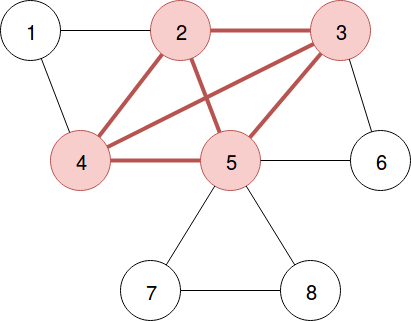
\includegraphics[width=0.25\textwidth]{images/clique.png}} & $\: \rightarrow \:$ & \raisebox{-.5\height}{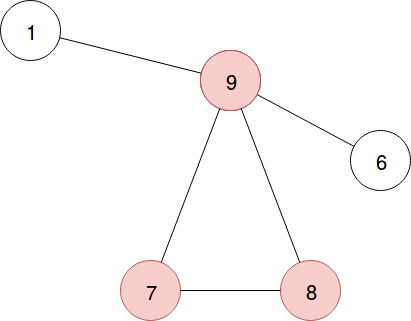
\includegraphics[width=0.25\textwidth]{images/firstReduce.png}} & $\: \rightarrow \:$ & \raisebox{-.5\height}{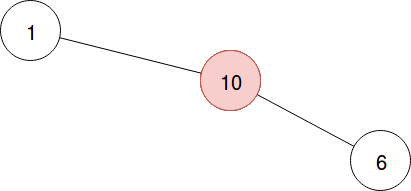
\includegraphics[width=0.25\textwidth]{images/secondReduce.png}}
\end{tabular}
\caption{A clique (left) can yet again be part of a clique (middle) after reduction. This would lead to the rightmost graph, which is no longer a good representation of the structure of the original graph (left).}\label{fig:clique}
\end{center}
\end{figure}

The search for cliques is rather straightforward.
After a vertex is selected (under the constraints) we depth-first search is done.
For every neighbour the vertex has it is checked that if these are added together a complete graph is created by these vertices and thus being a clique.
This process repeats itself until adding a new vertex no longer leads to having a clique.
Then the algorithm will backtrack to find all of the remaining cliques surrounding the originally selected vertex.

\begin{figure}[H]
\begin{center}
\begin{tabular}{ccc}
\raisebox{-.5\height}{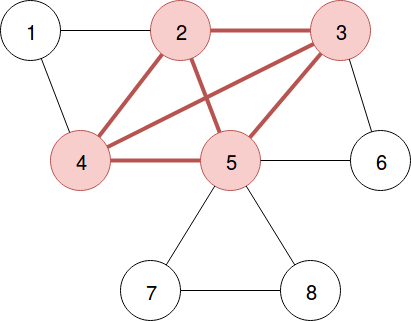
\includegraphics[width=0.30\textwidth]{images/clique.png}} & $\: \rightarrow \:$ & \raisebox{-.5\height}{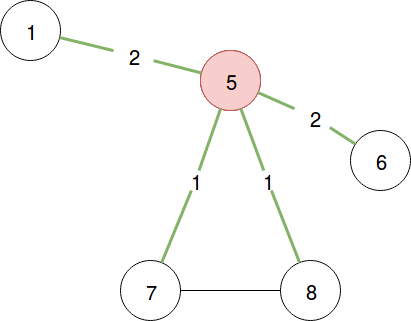
\includegraphics[width=0.30\textwidth]{images/reduced.png}}
\end{tabular}
\caption{The reduction of a clique to a single vertex and the adjustment of weights.}\label{fig:reduction}
\end{center}
\end{figure}

When all of the cliques surrounding a single vertex are found, the largest of them all will be selected for reduction.
With reduction it is meant that the vertices in the clique will be replaced by a single vertex in the graph.
But the underlying information of the edges will be retained by changing the value of the weigths on the corresponding edges.
The edges of which the weights will be adapted are those who are neighbouring to the vertices in the clique as can be seen in Fig. \ref{fig:reduction}.
Edges that have not been affected by any reduction will be considered to have the value of $1$ without explicitly stating it.

The result is a smaller graph.
If there are more edges between the vertices, then the probability of finding a clique also increases.
Highly connected networks will be the prime target for this method, because the largest reduction of size is to be expected in these cases.

The search space for the genetic algorithm is reduced. 
It will no longer be possible to assign individual elements in a clique to different communities.
The reasoning behind still applying this step is that when vertices are highly connected (for example form a clique) the likelihood that they are in the same communities increases. 
We note that this is not a lossless compression, but a lossy compression.

\subsection{Genetic Algorithm}
The method of a genetic algorithm is straighforward.
Define a representation, find a valid parent selection method and the corresponding operators (which are defined by their representation).
Choosing the right options is more difficult.
This section will therefor explain which options have been chosen for this report, all of these will come from the paper by Li et al \cite{Li2016}.

\subsubsection{Representation}
For the representation of a graph we are utilising a locus based representation (e.g. Fig. \ref{figure:locus}) as previously mentioned in Section \ref{sec:background}.
A graph will be represented by an array of vertex identifiers.
Having the value $5$ at index $3$ implies a connection $3 \rightarrow 5$.
Due to the limitations by the representation a vertex can only be in one community at the same time.
There are other representation that make this possible, but we have decided to limit our research to cases where this is not possible.

\subsubsection{Selection}
In the paper by Li et al \cite{Li2016} they suggest a network of agents to do the partner selection.
The network can be seen as a matrix of agents.
Only agents that are direct neighbours of the current agent are eligible partners.
From these neighbours the one with the highest fitness score will be chosen to reproduce with.
This is done to prevent agents from converging too quickly.

\begin{figure}[H]
\begin{center}
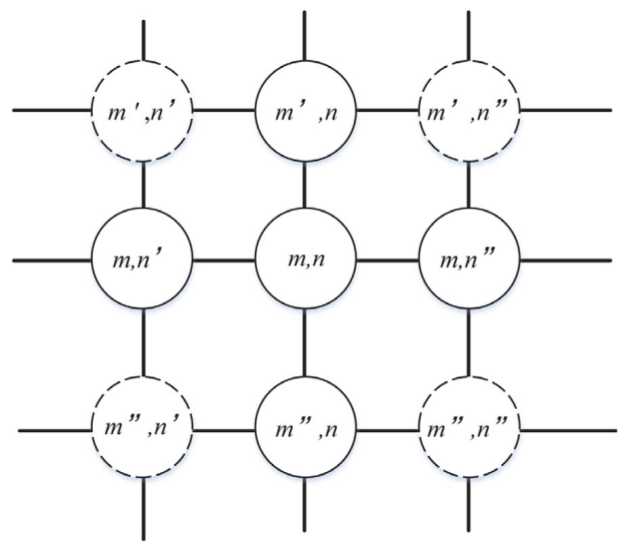
\includegraphics[width=0.5\textwidth]{images/neighbours.png}
\caption{An example of possible partners for an agent $m,n$ from the paper by Li. et al \cite{Li2016}.}\label{fig:neighbours}
\end{center}
\end{figure}
\newpage
As can be seen in the Fig. \ref{fig:neighbours} for an agent $m,n$ the neighbours are the following:\\
$neighbours_{m,n} = \lbrace L_{m',n},L_{m,n'},L_{m'',n},L_{m,n''} \rbrace$
\begin{center}
$ m' =
  \begin{cases}
    m-1       & \quad \text{if } m \neq 1\\
    L_{SIZE}  & \quad \text{if } m = 1\\
  \end{cases}\:,\qquad
n' =
  \begin{cases}
    n-1       & \quad \text{if } n \neq 1\\
    L_{SIZE}  & \quad \text{if } n = 1\\
  \end{cases}
$

$ m'' =
  \begin{cases}
    m+1       & \quad \text{if } m \neq L_{SIZE}\\
    1  & \quad \text{if } m = L_{SIZE}\\
  \end{cases}\:,\qquad
n'' =
  \begin{cases}
    n+1       & \quad \text{if } n \neq L_{SIZE}\\
    1  & \quad \text{if } n = L_{SIZE}\\
  \end{cases}
$
\end{center}

\subsubsection{Competition operator}
While dividing a network by using a locus-based representation, we can see that every vertex can only link to one other vertex and that in each community there can only be one loop.
The value of which a gene have to be different from all of the values from its current community.
If the value of an gene in an agent is changed, there are two possible outcomes.
Either that two communities will be merged together or that the community to which the gene belonged is split in two with one of them joining another community.

\subsubsection{Hybrid neighbourhood crossover}
In the paper by Li et al \cite{Li2016} a new crossover is introduced.
While doing crossover the best solution is never changed.
In practice this means that some of the values from the $MAX_{m,n}$ can be copied to the selected agent.
This is done to avoid losing good solutions and to avoid random recombinations.
This is completely different from the two-point crossover that was seen in section \ref{sec:background}.
There the two agents would exchange their information with each other. 


\subsubsection{Mutation}
\subsubsection*{Adaptive mutation}
In order to keep exploring the search space and retaining diversity in the population. We apply the neighbor-based mutation operator mentioned by C. Pizzuti \cite{Pizzuti2012}.
For each gene with some probability $p_{m}$ will it change its value to the allele of one of his neighbours.
This adaptive version of probability $p_{m}$ is used in \cite{Li2016}.
If no improvement is found, this parameter will increase to further stimulate the exploration of the search space.
Escaping local optima should be made easier by doing so.
After a certain amount of generations without improvements the algorithm will stop.
The exact function for the adaptive parameter is the following: \\
\begin{center}
$p_{m}' = (t/N_{s} + 1) \times p_{m}$
\end{center}

\subsection*{Self-Learning operator}
Excellent agents should be explored further.
To do so a local search method is applied.
Essentially a small-scale agent lattice is generated.
This is done by using the information in the selected agent and creating neighbours for this agent by using neighbour-based mutation.
This will create its own genetic algorithm and run for a certain amount of generations.
The best solution of this local genetic algorithm will replace the original one in the larger net.
All of the operators will be explained in more detail in section \ref{sec:implementation}.

